%%=============================================================================
%% Methodologie
%%=============================================================================

\chapter{Methodologie}
\label{ch:methodologie}

%% TODO: Hoe ben je te werk gegaan? Verdeel je onderzoek in grote fasen, en
%% licht in elke fase toe welke stappen je gevolgd hebt. Verantwoord waarom je
%% op deze manier te werk gegaan bent. Je moet kunnen aantonen dat je de best
%% mogelijke manier toegepast hebt om een antwoord te vinden op de
%% onderzoeksvraag.

%%\lipsum[21-25]
%%\section{Algemene opzet}
%%\label{sec:opzetexperiment}

Binnen dit experiment zullen er concreet 3 specifieke toestanden van een Android apparaat met elkaar vergeleken worden. Het eerste geval is een Android apparaat waarop er nog geen enkele wijziging is doorgevoerd. Deze staat dus nog gelijk met de fabrieksinstellingen van het apparaat. Bij het tweede geval zijn de instellingen zo aangepast om de dataverzameling van Google te minimaliseren. Bij deze toestand wordt er optimaal gebruik gemaakt van de mogelijkheden die Google en het Android besturingssysteem zodat er zo min mogelijk data wordt verzameld. In het derde geval zullen er methodes gebruikt worden, die niet direct door Google of Android zelf worden ondersteund, om zo Google volledig te proberen elimineren van het apparaat.

Bij deze drie gevallen zal er in detail beschreven worden welke stappen precies moeten worden genomen om de testtoestand van het apparaat te bekomen. Daarna zal het internetverkeer van elk geval geanalyseerd worden gedurende 1 uur. Concreet wordt er hier geregistreerd hoeveel keer er gemiddeld data wordt verstuurd naar specifieke internet domeinen van Google.

\section{Testapparaat}
\label{sec:testapparaat}
Het experiment zal plaatsvinden op een Oneplus 5 apparaat (model nr. ONEPLUS A500). Dit apparaat draait op een aangepaste versie van Android, genaamd OxygenOS. OxygenOS is een Android ROM die gekend is voor het toevoegen van configureerbaarheid en handige functies, terwijl de 'look and feel' grotendeels gelijkt blijft in vergelijking met stock Android. De bloatware die hierbinnen wordt meegeleverd is ook minimaal. De laatste versie van OxygenOS die beschikbaar is op het moment van schrijven, is OxygenOS 9.0.5, die verderbouwt op Android 9.0, ofwel Android Pie.

\section{Testgevallen}
\label{sec:testgevallen}
% TODO ALLE SETTINGS AAN locatie bluetooth wifi 4g

In deze sectie zullen de verschillende testgevallen in detail besproken worden.

\subsection{Testgeval 1: Android met fabrieksinstellingen}
\label{sec:testgeval1}
Binnen dit geval zal gebruik gemaakt worden van een Android apparaat waarbij buiten de initiële setup geen wijzigingen zijn gebeurd. Om in deze toestand terecht te raken zal er binnen OxygenOS gebruik worden gemaakt van de functie 'Alle gegevens wissen (fabrieksinstellingen terugzetten)'. Dit is te vinden in de 'Instellingen' applicatie, onder 'Systeem' >  'Opties voor resetten' > 'Alle gegevens wissen (fabrieksinstellingen terugzetten)'. Wanneer er naar het juiste scherm genavigeerd is, wordt er ook gekozen om de interne opslag te wissen, zoals te zien in figuur \ref{fig:fabrieksinstellingen}.

\begin{figure}
    \centering
    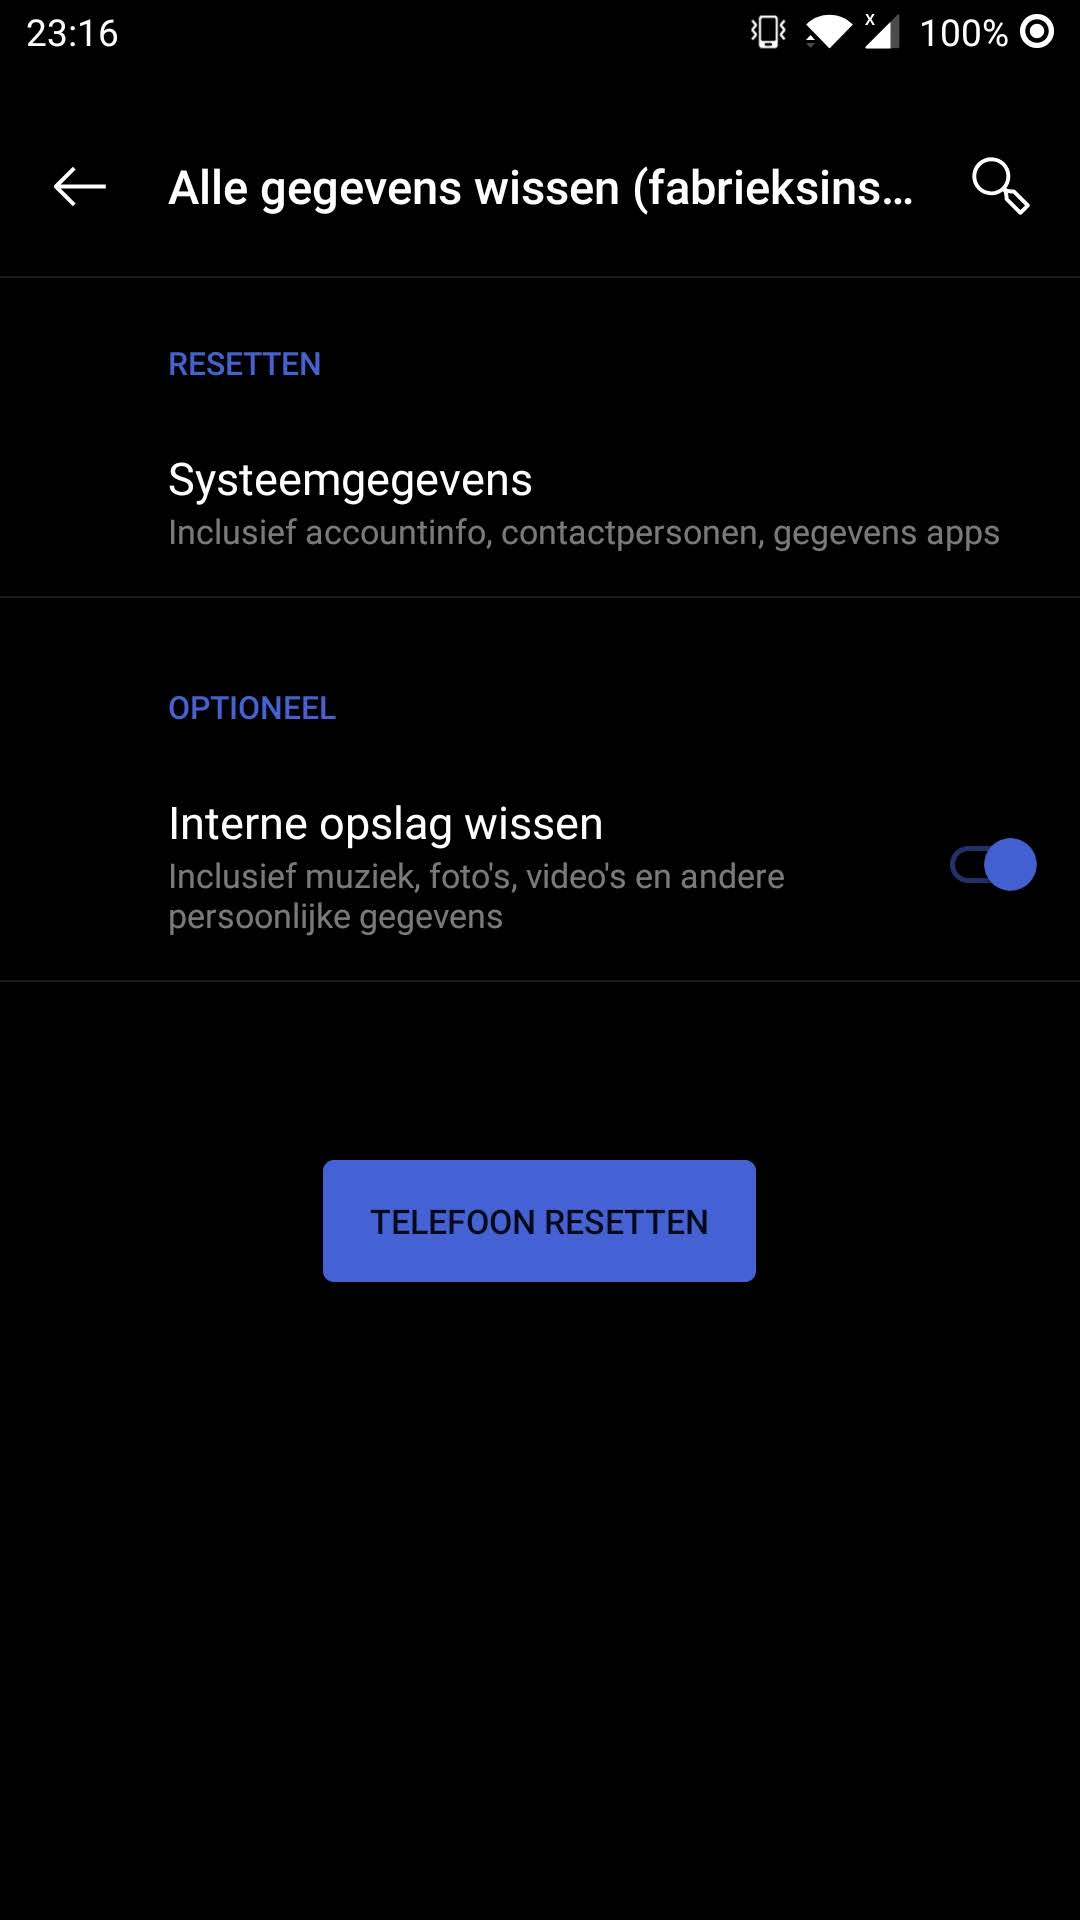
\includegraphics[width=0.4\textwidth]{img/fabrieksinstellingen.jpg}
    \caption{Screenshot van het scherm waar alle gegevens gewist kunnen worden en de fabrieksinstellingen kunnen worden teruggezet}
    \label{fig:fabrieksinstellingen}
\end{figure}


\subsection{Testgeval 2: Android met aangepaste instellingen}
\label{sec:testgeval2}

%TODO testgeval 2

\subsection{Testgeval 3: Volledig aangepaste Android}
\label{sec:testgeval3}

%TODO testgeval 3

\section{Meting software}
\label{sec:metingsoftware}
Het verzamelen van data die de netwerkactiviteit van het apparaat beschrijft, zal op een gelijkaardige manier worden gedaan zoals in het onderzoek door \cite{schmidt_google-data-collection}, wat ook in de litatuurstudie werd besproken. Om exact te kunnen zien welke data er precies binnenkomt en buitengaat via het internet op het apparaat, is er extra software nodig. Deze optie wordt namelijk niet gegeven door het Android besturingssysteem zelf. De software die wij gebruiken moet voldoen aan enkele voorwaarden:
\begin{itemize}
    \item De verkregen data moet kunnen worden geëxporteerd naar een bruikbaar formaat.
    \item De software mag geen aanpassing maken aan of vereisen van het apparaat.
    \item De software moet de gevraagde data verzamelen zonder dat deze wordt beïnvloed door de software zelf.
\end{itemize}
Er bestaan reeds veel applicaties die rechstreeks vanaf het Android apparaat deze data kan verzamelen. Velen hiervan vallen al direct weg, aangezien ze root toegang vereisen. De 'geroote' toestand is namelijk een voorwaarde van de testgevallen, waardoor we deze doorheen de gevallen niet ingeschakeld kunnen houden.%TODO VERDER
